
\documentclass[handout]{beamer}
\usepackage{pgfpages}
%\documentclass{beamer}
%\usepackage{beamerthemesplit}

\def\ce#1{\centerline{#1}}
\def\no{\noindent} 
\def\nl{\newline}
% -------
 \def\cblack{\color{black}}
 \def\cb{\color{blue}}
 \def\cred{\color{red}}
 \def\cy{\color{yellow}}
 \def\cg{\color{cyan}}
% -------
 \def\bs{\end{frame}\begin{slide}}
 \def\bi{\begin{itemize}[<+-| alert@+>]} 
 \def\ei{\end{itemize}}
 \def\i{\item} 
 
\def\t{\theta} 
\def\l{\lambda} 
\def\d{\delta} 

 \def\cblack{\color{black}}
 \def\cb{\color{white}}
 \def\cred{\color{yellow}}
 \def\cy{\color{yellow}}
 \def\cg{\color{green}}
% -------
\def\bs{\end{frame}\begin{slide}}
 \def\bi{\begin{itemize}[<+-| alert@+>]} 
 \def\ei{\end{itemize}}
 \def\i{\item} 


\def\t{\theta} 
\def\T{\Theta} 
\def\l{\lambda} 
\def\d{\delta} 
\def\e{\varepsilon} 
\def\s{\sigma} 
\def\ss{\sigma^2} 
\def\Sy{S_{yy}} 
\def\SS{\textsf{SS}} 
\def\N{\textsf{N}} 
\def\NG{\textsf{NG}} 
\def\Ga{\textsf{G}} 
\def\Sx{S_{xx}}
\def\Sxy{S_{xy}}
\def\ha{{\hat\alpha}}
\def\hb{{\hat\beta}}
\def\hy{{\hat y}}
\def\bx{\bar x}
\def\by{\bar y}

 \def\bi{\begin{itemize}} 
 \def\ei{\end{itemize}}
 \def\i{\item} 
 \def\tr{\textsf{tr}} 
\def\Wishart{\textsf{Wishart}}


\title{STA 360/601: Bayesian and Modern Statistics}

\subtitle{Lecture 10: Multivariate Gaussian models}

\author{Jeff Miller}

\institute{Department of Statistical Science, Duke University}

\date{Friday, September 26, 2014}

\begin{document}

\frame{\titlepage}

%\section[Outline]{}
%\frame{\tableofcontents}



\begin{frame}
\frametitle{Bivariate Gaussian distribution}
\begin{itemize}[<+-| alert@+>]
    \item $Y = (Y_1,Y_2)' \sim N_2( \mu, C)$ ({\em bivariate Gaussian}) has pdf
$$f(y) = (2\pi)^{-1}|C |^{-1/2} \exp\bigg\{ -\frac{1}{2} (y - \mu)'C^{-1}(y - \mu) \bigg\},$$
where $| A | = |\det A|$

\item Gaussian distribution is parameterized by mean $\mu$ and covariance matrix $C$

\item $\mu = \mbox{E}( Y ) = (\mbox{E}(Y_1), \mbox{E}(Y_2))' = (\mu_1,\mu_2)' $ is the mean (first moment) 

\item $C = \mbox{cov}( Y )$ = covariance matrix - characterizes co-variability in the different elements of $Y$

\item ``Normal'' = ``Gaussian''
\end{itemize}
\end{frame}

\begin{frame}
\frametitle{Covariance matrix}
\begin{itemize}[<+-| alert@+>]
    \item Note that $Y=(Y_1,Y_2)'$ is a bivariate random variable, and its components may be linearly dependent

\item The bivariate normal distribution allows this dependence to range from perfectly negatively correlated to zero
(independent) to perfectly positively correlated

\item The covariance matrix $C$ encodes this dependence and the marginal variances of $Y_1$ and $Y_2$

\item Writing $C = ( C_{jk} )$ with $C_{jk}$ denoting the $(j,k)$th element of the covariance matrix, we have
$$C_{11} = \mbox{var}( Y_1 ),\quad C_{22} = \mbox{var}( Y_2 ),\quad 
C_{12}=C_{21} = \mbox{cov}( Y_1,Y_2)$$
\end{itemize}
\end{frame}

\begin{frame}
\frametitle{Covariance matrix}
\begin{itemize}[<+-| alert@+>]
    \item The covariance between $Y_1$ and $Y_2$ is defined as 
        $$\mbox{cov}( Y_1,Y_2) = \mbox{E}(Y_1 Y_2) - \mbox{E}(Y_1)\mbox{E}(Y_2).$$

    \item The correlation coefficient between $Y_1$ and $Y_2$ is defined as 
$$\rho_{12} = \frac{ \mbox{cov}(Y_1,Y_2) }{ \sqrt{ \mbox{var}(Y_1) }\sqrt{ \mbox{var}(Y_2)} } 
= \frac{ C_{12} }{ \sigma_1 \sigma_2 },$$
where $\sigma_1 = \sqrt{C_{11}}$ and $\sigma_2 = \sqrt{C_{22}}$.

\item $-1 \le \rho_{12} \le 1$ and the correlation coefficient is free of the measurement units
\end{itemize}
\end{frame}

\begin{frame}
\frametitle{Plotting bivariate Gaussian - contour plot}
\begin{figure}[!t]
\centerline{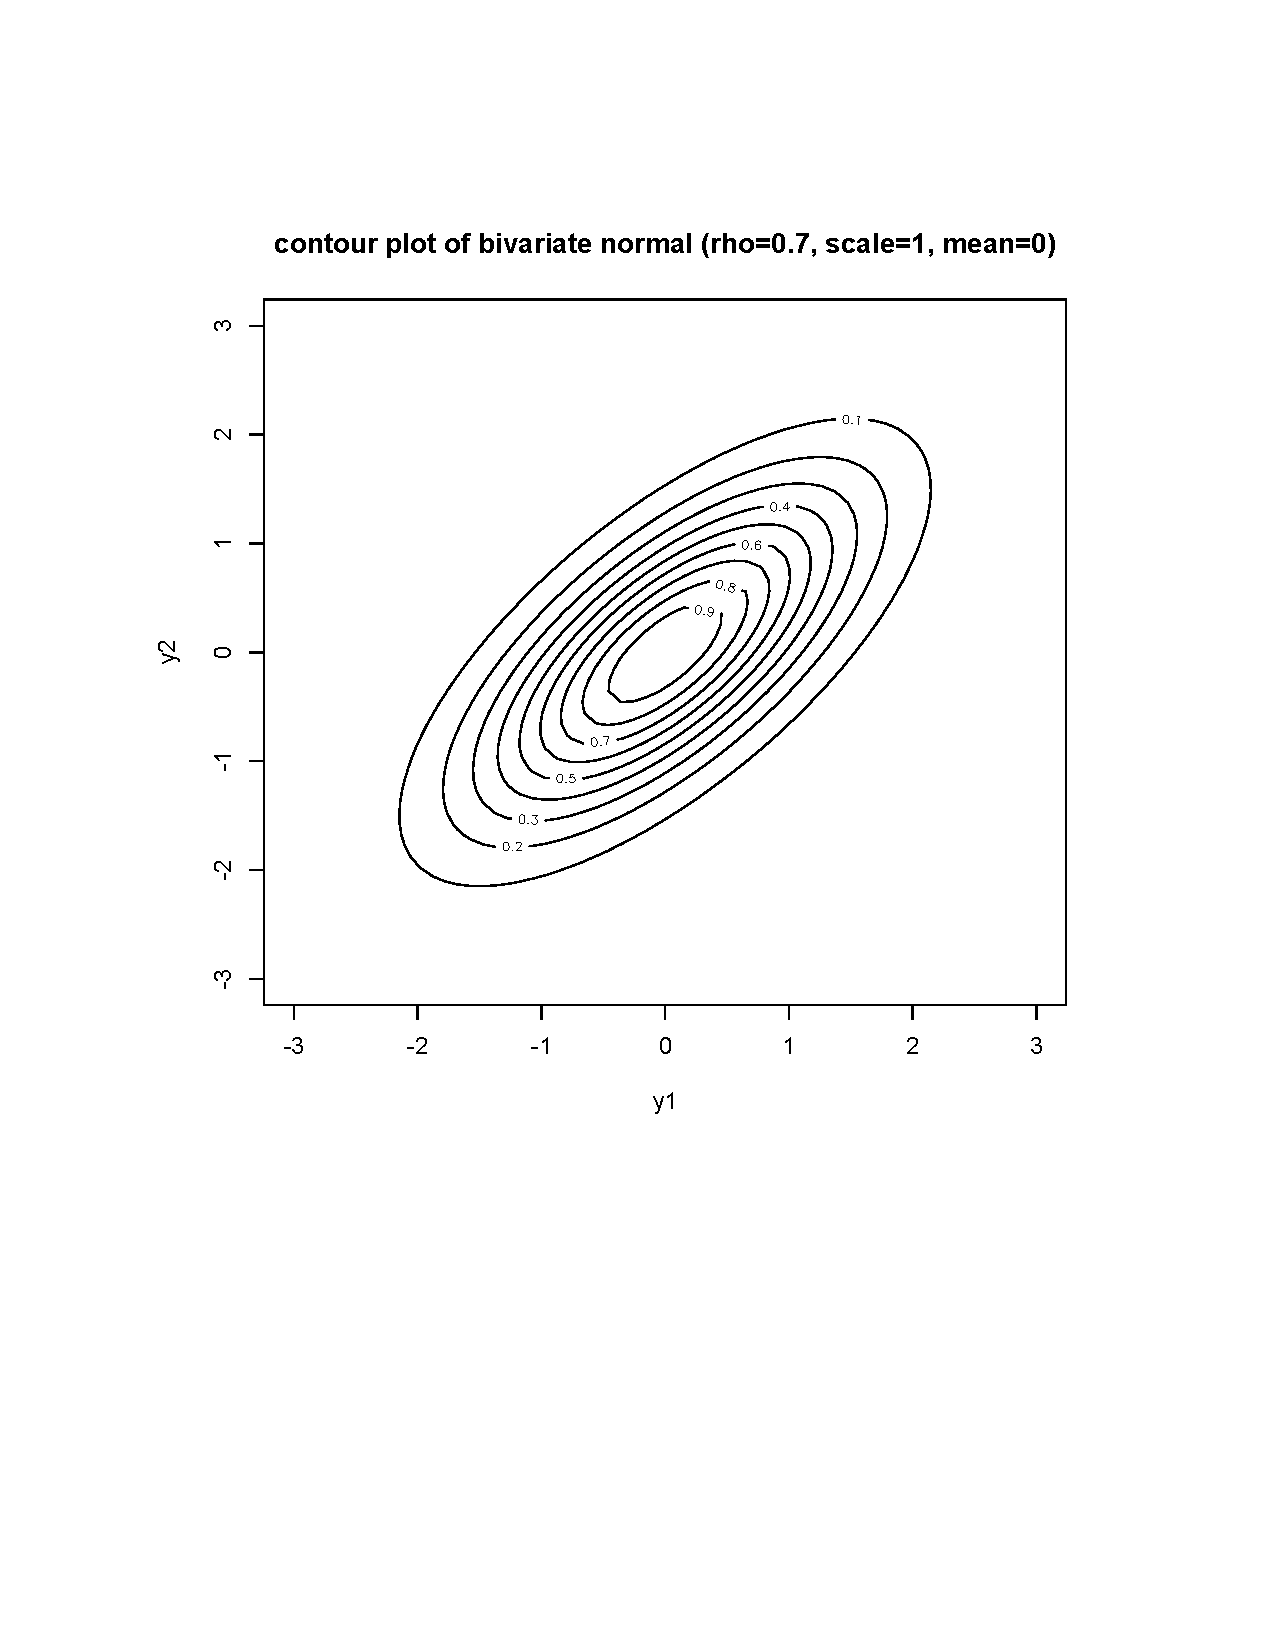
\includegraphics[width=9cm]{lecture10fig1}}
\end{figure}
\end{frame}

\begin{frame}
\frametitle{Plotting bivariate Gaussian - heat plot}
\begin{figure}[!t]
\centerline{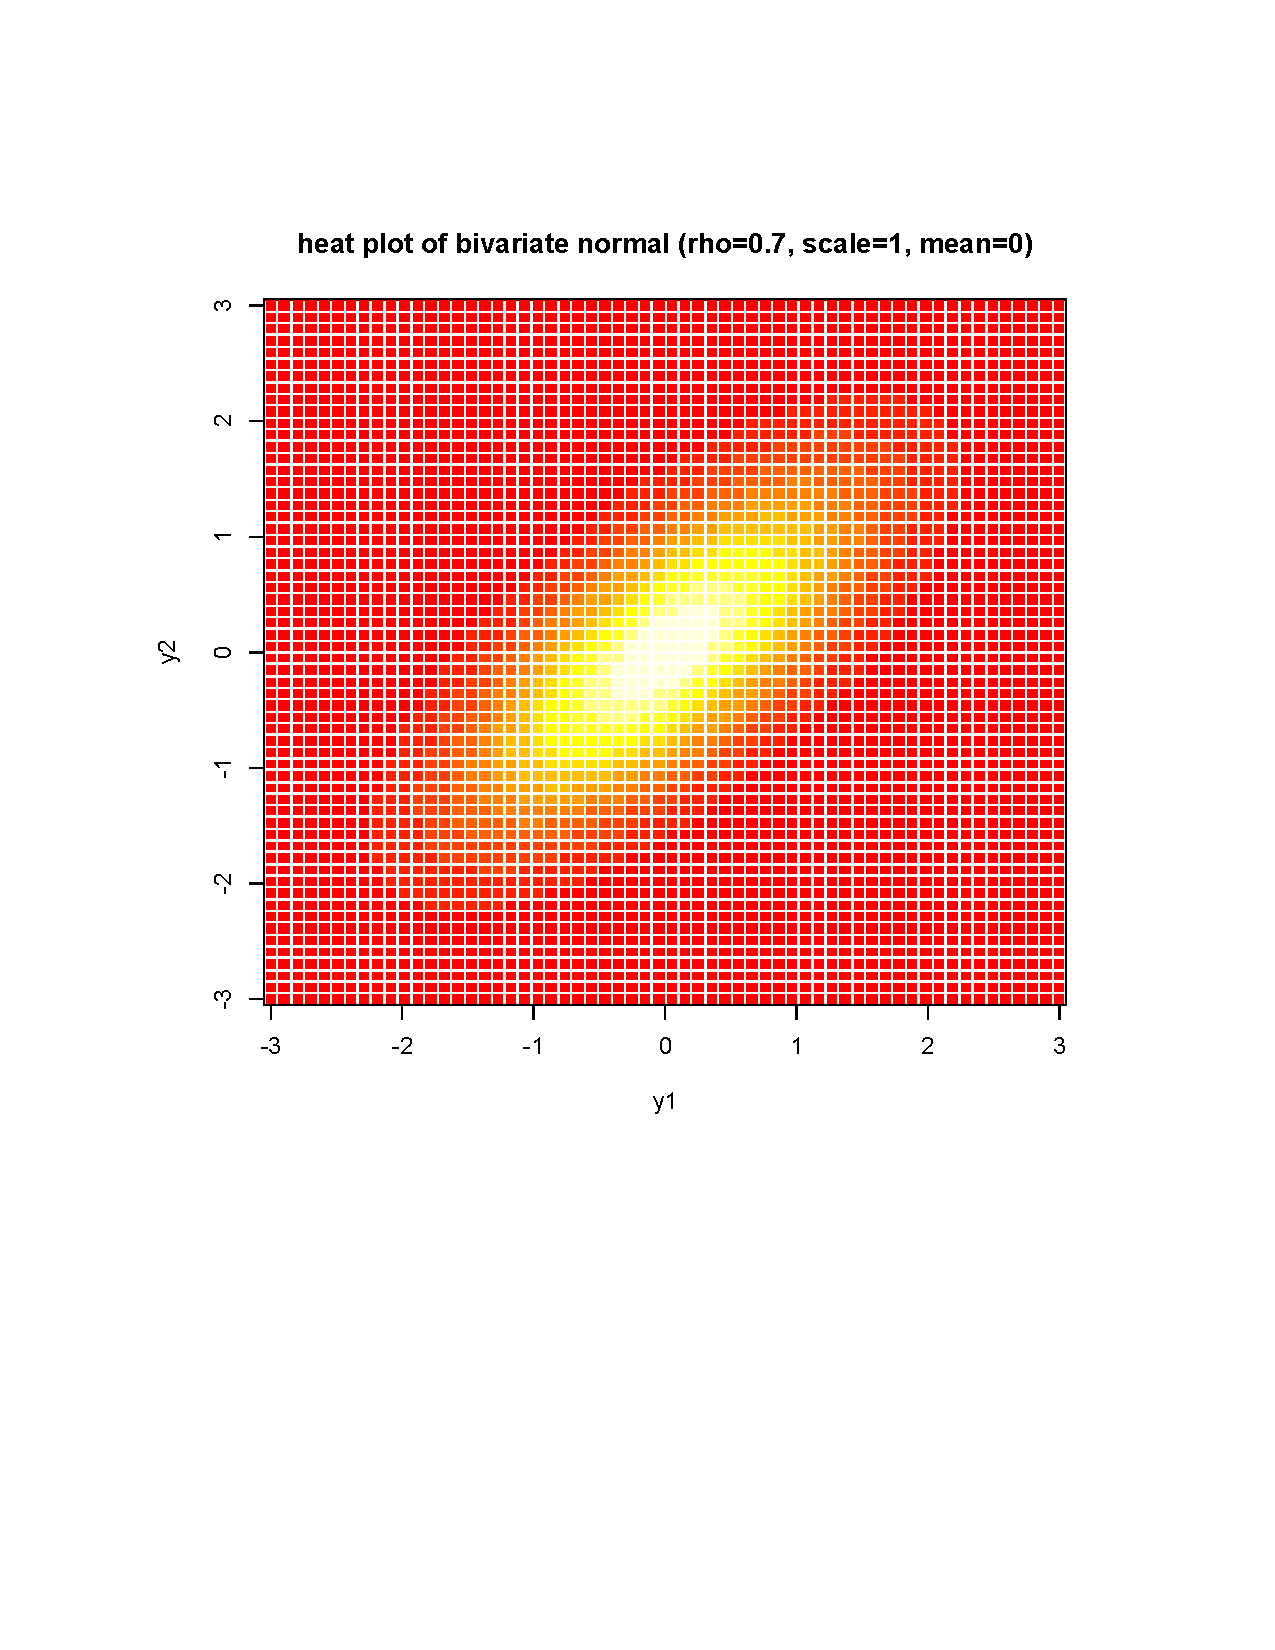
\includegraphics[width=9cm]{lecture10fig2}}
\end{figure}
\end{frame}

\begin{frame}
\frametitle{Plotting bivariate Gaussian - 3d perspective plot}
\begin{figure}[!t]
\centerline{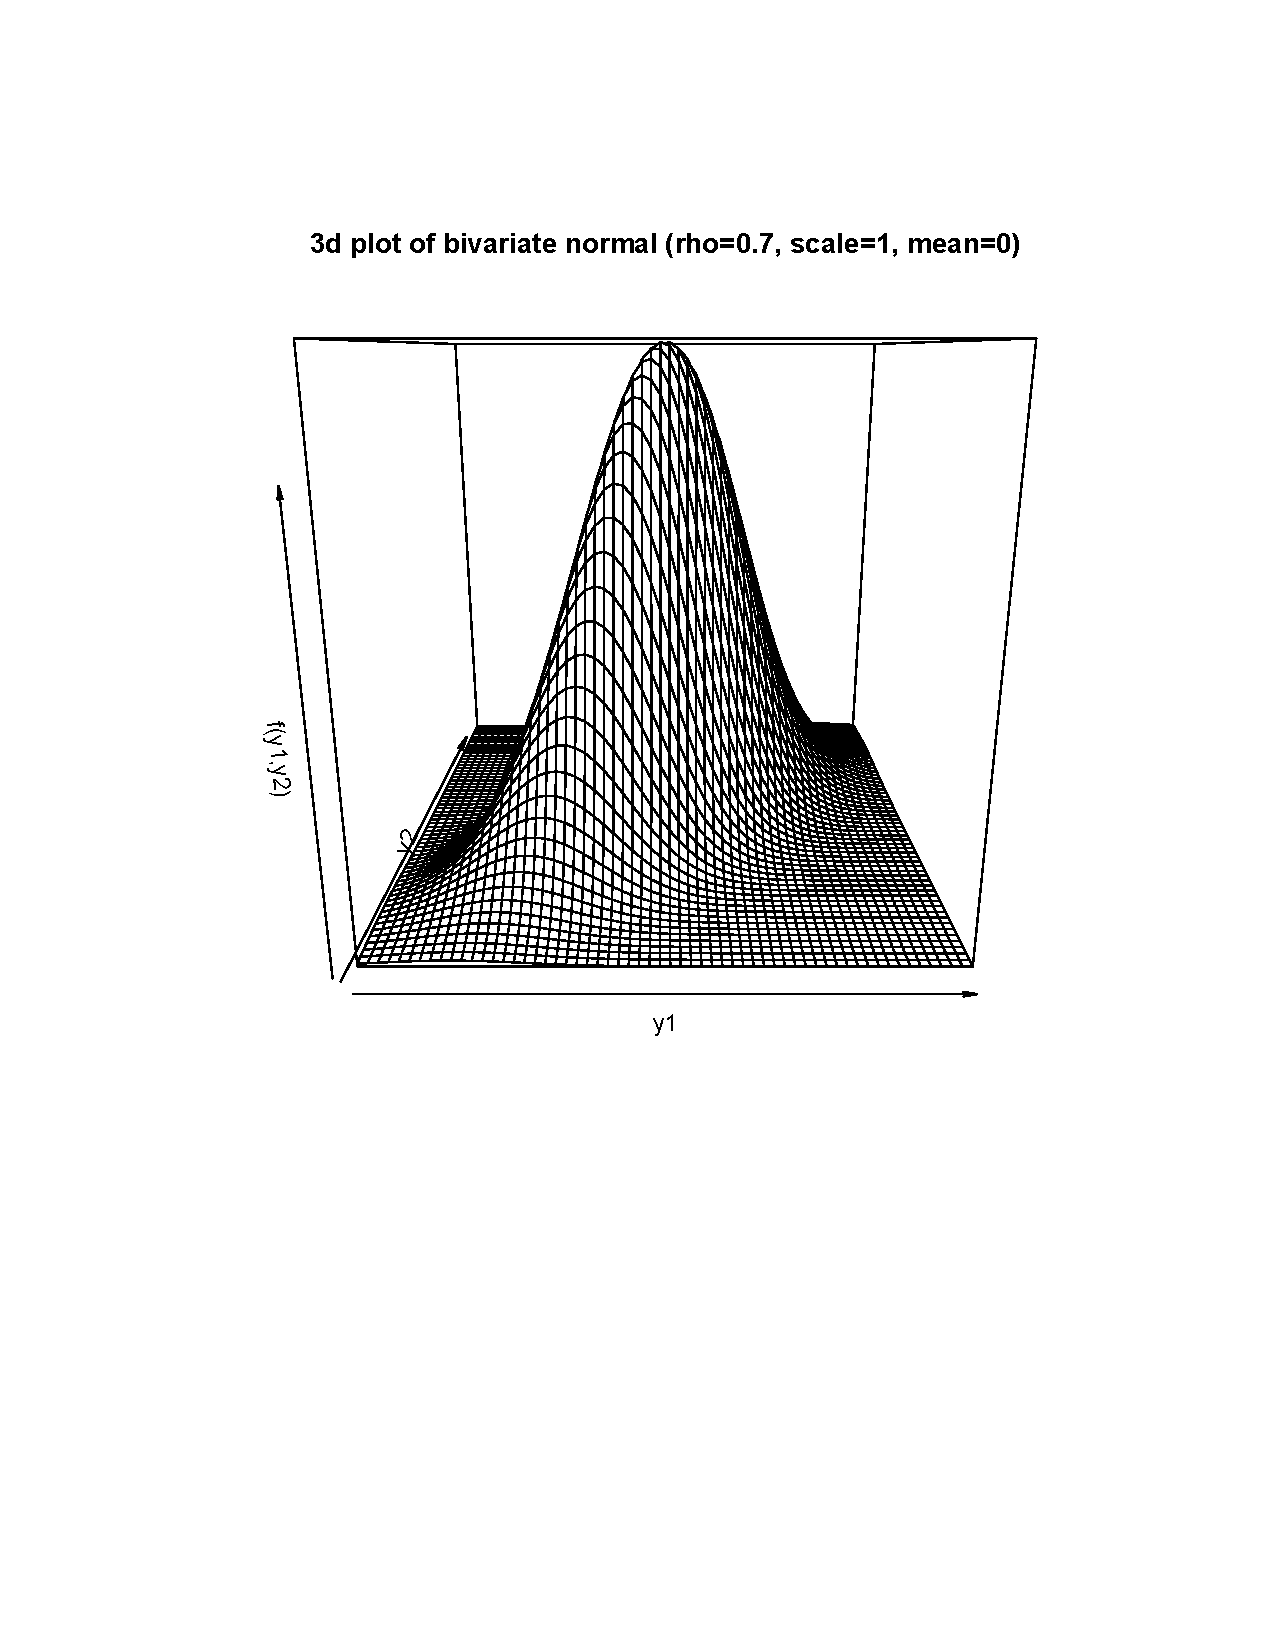
\includegraphics[width=9cm]{lecture10fig3}}
\end{figure}
\end{frame}

\begin{frame}
\frametitle{Contour plot of spherical Gaussian}
\begin{figure}[!t]
\centerline{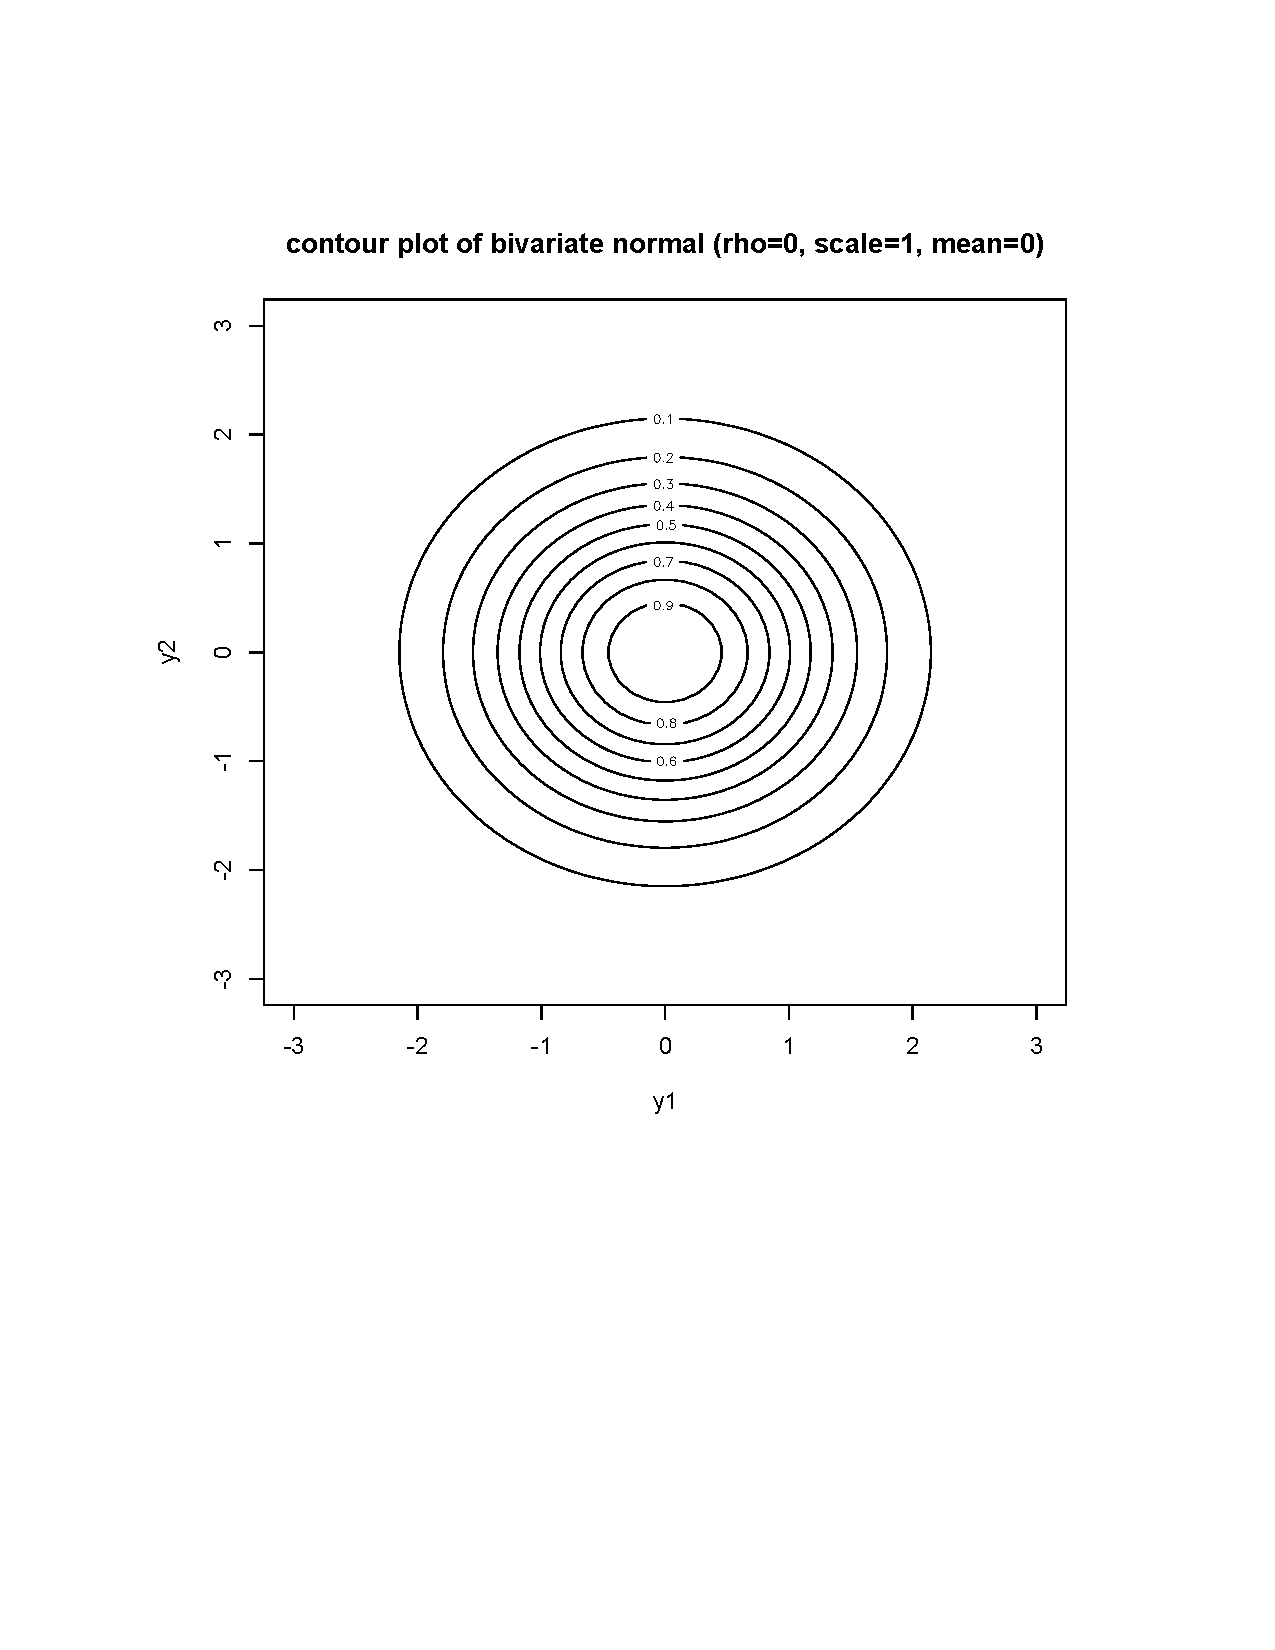
\includegraphics[width=9cm]{lecture10fig4}}
\end{figure}
\end{frame}

\begin{frame}
\frametitle{Contour plot - high negative correlation}
\begin{figure}[!t]
\centerline{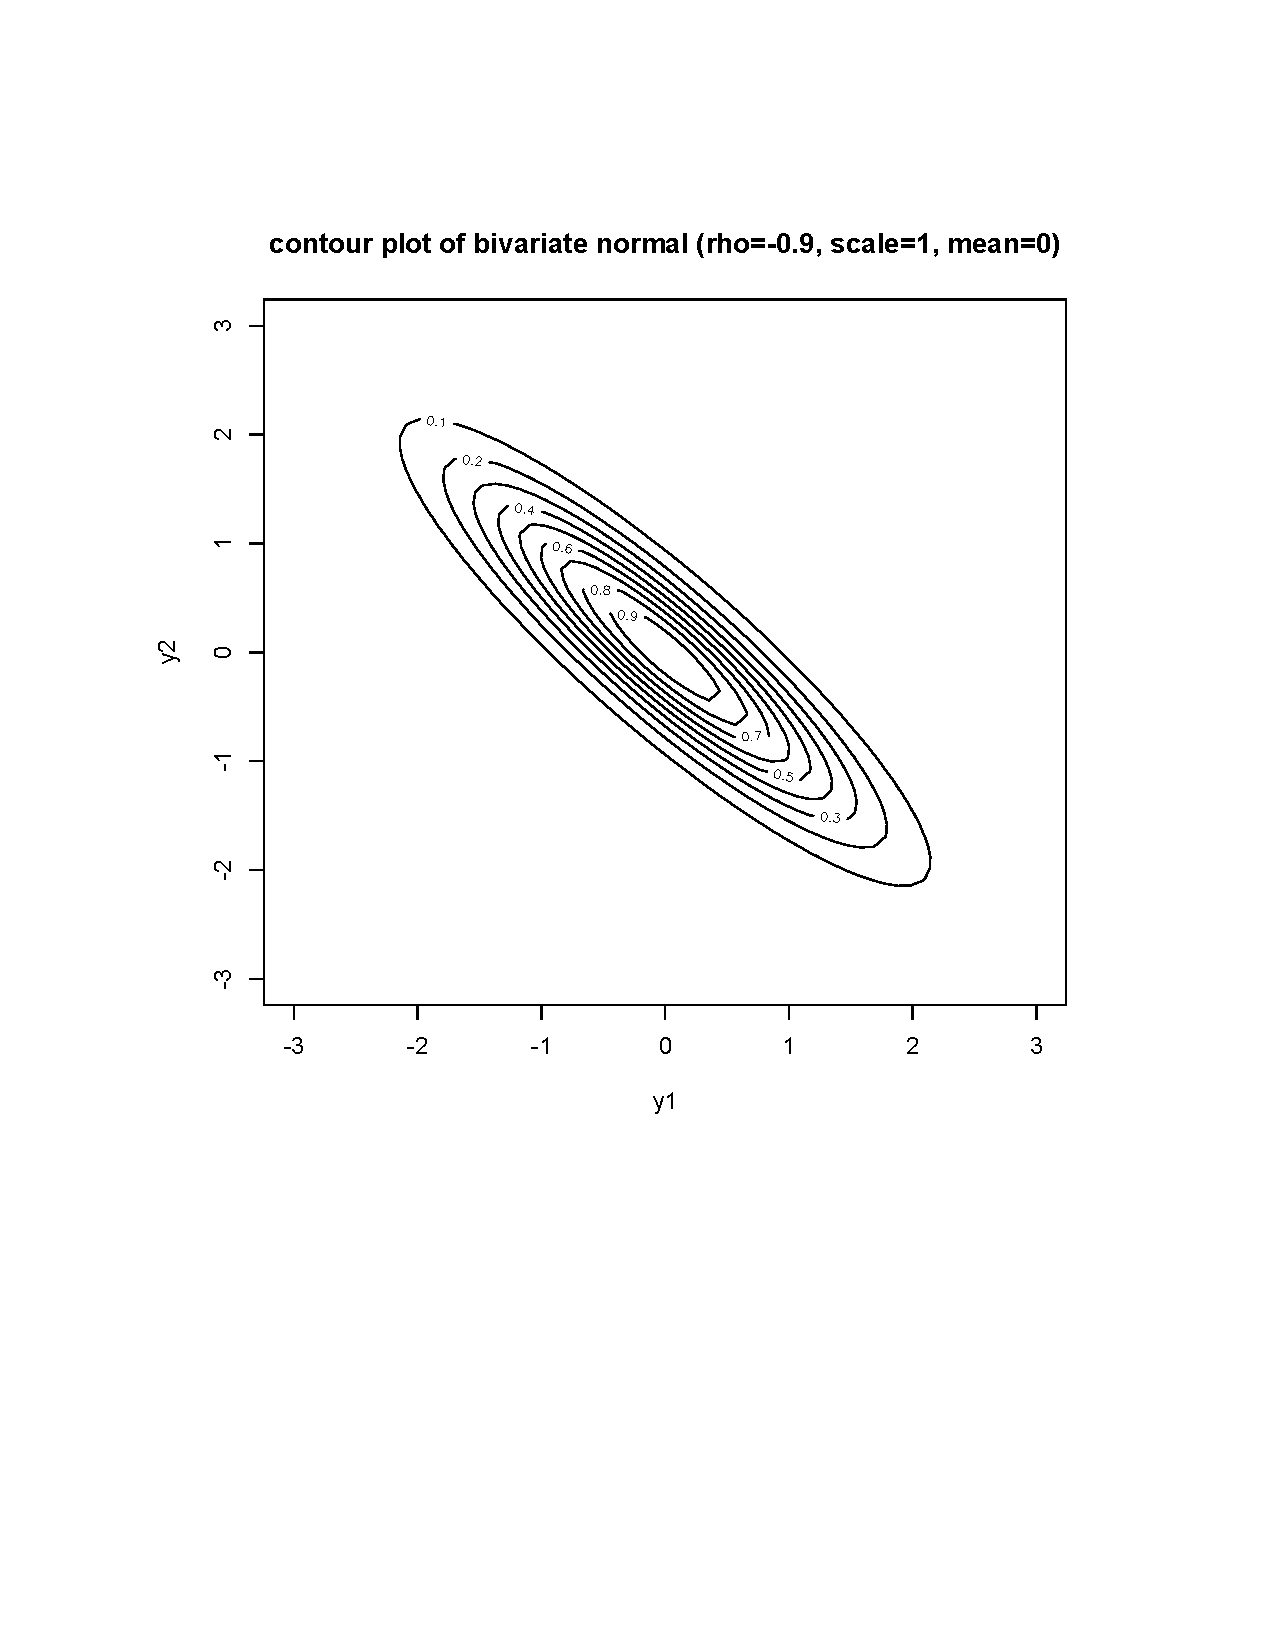
\includegraphics[width=9cm]{lecture10fig5}}
\end{figure}
\end{frame}

\begin{frame}
\frametitle{General Multivariate Gaussian distribution}
\begin{itemize}[<+-| alert@+>]
    \item Straightforward to generalize to multiple dimensions: the pdf of the $p$-dimensional Gaussian $N(\mu,C)$ is
$$f(y) = (2\pi)^{-p/2}|C|^{-1/2} \exp\bigg\{ -\frac{1}{2} (y - \mu)'C^{-1}(y - \mu) \bigg\},$$
where $y = (y_1,\ldots,y_p)'$

\item $\mu$ is now a $p \times 1$ vector and $C$ is a $p \times p$ matrix 

\item Can obtain as follows: if $Z=(Z_1,\ldots,Z_p)'$ with $Z_i\stackrel{iid}{\sim} N(0,1)$ then $Y = C^{1/2}Z+\mu\sim N(\mu,C)$.

\item Interpretation is maintained in multivariate case: $(j,k)$th element of $C$ is $\mbox{cov}(Y_j,Y_k)$

\item Special property of multivariate normal:   $Y_j$ and $Y_k$
    are independent iff they are uncorrelated (i.e., $\rho_{jk}=0$)
\end{itemize}
\end{frame}

\begin{frame}
\frametitle{Conditional Distributions}
\begin{itemize}[<+-| alert@+>]
\item Let $Y = (Y_a', Y_b')'$ with $Y_a$ the first $q$ elements of $Y$ and $Y_b$ the remaining $p-q$ elements

\item Suppose $Y  \sim N_p( \mu, C)$ with 
$$\mu = \left( \begin{array}{c}
\mu_a \\
\mu_b
\end{array}\right)\quad \mbox{and}\quad
C = \left( \begin{array}{cc}
C_{aa} & C_{ab} \\
C_{ba} & C _{bb} 
\end{array} \right),$$
where $\mu_a$ is $q \times 1$, $\mu_b$ is $(p-q) \times 1$, $C_{aa}$ is $q \times q$, $C_{bb}$ is $(p-q) \times (p-q)$
 
\item Then the conditional distribution of $Y_a$ given $Y_b=y_b$ is
$$(Y_a|Y_b=y_b) \sim N_q\big( \mu_a + C_{ab}C_{bb}^{-1}(y_b-\mu_b), C_{aa}-C_{ab}C_{bb}^{-1}C_{ba} \big).$$
\end{itemize}
\end{frame}

%\begin{frame}
%\frametitle{Conditional Distributions - Linear Regression}
%\begin{itemize}[<+-| alert@+>]
%\item Previous equation implies multivariate linear regression
%\begin{eqnarray}
%\mbox{E}(y_1|y_2=a) = \mu_1^* + \beta a,\quad \mbox{V}(y_1|y_2=a) = \Sigma_1^*, \nonumber
%\end{eqnarray}

%\item The intercept is $\mu_1^*=\mu_1 - C_{12}C_{22}^{-1}\mu_2$ 

%\item The matrix of regression coefficients $\beta = C_{12}C_{22}^{-1}$

%\item In bivariate case in which $p=2,q=1$, we have 
%\begin{eqnarray}
%(y_1|y_2=a) \sim N\bigg( \mu_1 + \frac{\sigma_1}{\sigma_2}\rho(a-\mu_2), (1-\rho^2)\sigma_1^2 \bigg), \nonumber
%\end{eqnarray}
%where $\rho = \mbox{cor}(y_1,y_2)$.
%\end{itemize}
%\end{frame}
 
\begin{frame}
\frametitle{Bayesian inference for the mean $\mu$}
\begin{itemize}[<+-| alert@+>]
\item For data $Y_i = (Y_{i1},\ldots,Y_{ip})' \sim N( \mu, C)$ the likelihood is $\propto$
$$|C|^{-n/2}\exp\bigg\{ -\frac{1}{2}\sum_{i=1}^n (y_i - \mu)' C^{-1}(y_i - \mu) \bigg\}$$

\item Under a multivariate Gaussian prior $\mu \sim N_p( \mu_0, C_0 )$, the conditional 
posterior distribution of $\mu$ is 
$$( \mu | C, y_{1:n}) \sim N_p( \hat{\mu}, \hat{C}),$$

where
$$\hat{C} = (C_0^{-1} + n C^{-1})^{-1},$$ 
and
$$\hat{\mu}=\hat{C}( C_0^{-1}\mu_0 + n C^{-1}\overline{y} ).$$

\item $\hat{C}$ is the \underline{conditional} posterior covariance of $\mu$. Note that 
    ``learning'' is more rapid when the precision (inverse covariance) $C^{-1}$ is ``big''.

\item $\hat{\mu}$ is the \underline{conditional} posterior mean of $\mu$.
\end{itemize}
\end{frame}


\begin{frame}
\frametitle{What about inference for the covariance matrix?}
\begin{itemize}[<+-| alert@+>]
\item In the univariate case, $Y_i \sim N(\mu,\sigma^2)$, an inverse-gamma prior is commonly 
chosen for the variance $\sigma^2$

\item This is equivalent to a gamma prior for the precision $\lambda = 1/\sigma^{2}$

\item In the multivariate Gaussian case, we have a covariance matrix $C$ instead of a
scalar

\item It would be nice to have a matrix-valued extension of the inverse-gamma that would be conjugate
\end{itemize}
\end{frame}

\begin{frame}
\frametitle{Positive definite \& symmetric}
\begin{itemize}[<+-| alert@+>]
\item One complication is that the covariance $C$ must be symmetric and {\em positive definite} (posdef)

\item i.e., $C=C'$ and $x' C x > 0$ for all $x \in \mathbb{R}^p$ s.t.\ $x\neq 0$

\item Note that this ensures that the diagonal elements of $C$ (corresponding to the marginal variances $\sigma_j^2$) 
are positive

\item Also, ensures that the correlation coefficients for each pair of variables are between $-1$ and $1$.

\item Prior for $C$ must assign probability $1$ to the set of symmetric positive definite matrices
\end{itemize}
\end{frame}

\begin{frame}
\frametitle{Constructing a random posdef matrix}
\begin{itemize}[<+-| alert@+>]
\item It seems daunting to directly specify a prior with appropriate support 

\item But consider the following:

\item Sample $Z_\ell \stackrel{iid}{\sim} N_p( 0, U )$ for $\ell=1,\ldots,\nu$, where $U$ is a $p\times p$ symmetric posdef matrix

\item Let $\Lambda = \sum_{\ell=1}^{\nu} Z_\ell Z_\ell'$, i.e., $$\Lambda_{jk} = \sum_{\ell=1}^{\nu} Z_{\ell j} Z_{\ell k}$$

\item The distribution of $\Lambda$ is called Wishart, and denoted $\mbox{W}_p(\nu,U)$

\item $\nu$ = ``degrees of freedom'', $U$ = ``scale matrix''
\end{itemize}
\end{frame}

\begin{frame}
\frametitle{Wishart - some properties}
\begin{itemize}[<+-| alert@+>]
\item $\Lambda$ is always symmetric

\item If the degrees of freedom $\nu \geq p$, then $\Lambda$ is posdef with probability 1

\item $\mbox{E}( \Lambda ) = \nu U$

\item Hence, $U$ can be viewed as a scaled version of the mean of $\Lambda$

\item The pdf of $\Lambda \sim \mbox{W}_p( \nu, U)$ is $\propto$
$$ | \Lambda |^{\frac{\nu-p-1}{2}} e^{ -\frac{1}{2} \mbox{tr}( U^{-1}\Lambda)}$$
where $\mbox{tr}(\cdot)$ is the {\em trace} function (sum of diagonal elements)

\item In the univariate case in which $p=1$, this reduces to 
    $$\lambda^{\nu/2 - 1} e^{-\frac{1}{2}u^{-1}\lambda } \propto \mbox{Ga}(\lambda|\nu/2, 1/(2 u))$$

\end{itemize}
\end{frame}

%\end{document}

\begin{frame}
\frametitle{Wishart - some comments}
\begin{itemize}[<+-| alert@+>]
\item Wishart provides a conditionally-conjugate prior for the precision matrix $\Lambda = C^{-1}$
in a multivariate normal model

\item Wishart is a multivariate generalization of the gamma prior for a scalar precision (1/variance)

\item What about the covariance matrix?
\end{itemize}
\end{frame}

\begin{frame}
\frametitle{Inverse Wishart}
\begin{itemize}[<+-| alert@+>]
\item When $\Lambda \sim \mbox{W}_p(\nu,U)$, $\nu\geq p$, the distribution of $\Lambda^{-1}$ is called {\em Inverse Wishart}, and denoted $\mbox{IW}_p(\nu,S)$, where $S=U^{-1}$.
\item $C=\Lambda^{-1}$ is symmetric posdef with probability 1
\item The pdf of $C \sim \mbox{IW}_p( \nu, S)$ is $\propto$

    $$|C|^{-(\nu+p+1)/2} e^{ -\frac{1}{2}\mbox{tr}( S C^{-1}) }$$

\item $\nu$ = ``degrees of freedom'', $S$ = ``scale matrix'' (posdef)

\item $\mbox{E}(C) = \frac{1}{\nu-p-1} S$

\item If we have a prior guess $C_0$ for $C$ then we might choose $S=(\nu-p-1)C_0$
\item Under this choice, $\mbox{E}( C ) = C_0$, and $\nu = p+2$ would correspond to a vague prior

\item The inverse Wishart is a conditionally-conjugate prior for the multivariate normal covariance and provides
a multivariate generalization of the inverse-gamma
\end{itemize}
\end{frame}

\begin{frame}
\frametitle{Bayesian inference for the covariance matrix}
\begin{itemize}[<+-| alert@+>]
    \item Suppose $C \sim \mbox{IW}_p(\nu,S)$ and $Y_1,\ldots,Y_n\sim N_p(\mu,C)$
    \item Letting $S_{y,\mu} =\sum_{i=1}^n (y_i - \mu)(y_i - \mu)'$, we have
\begin{align*}
f(C|\mu,y_{1:n}) & \propto |C|^{-(\nu+p+1)/2} e^{ -\mbox{tr}( S C^{-1})/2 } 
                      |C|^{-n/2} e^{ -\mbox{tr}( S_{y,\mu} C^{-1} )/2 } \\
                      %& = |C|^{-(\nu+n+p+1)/2} e^{-\mbox{tr}((S+S_{y,\mu})C^{-1})/2}
                      & = |C|^{-(\hat{\nu}+p+1)/2} e^{-\mbox{tr}(\hat{S} C^{-1})/2}
\end{align*}
where 
$$\hat{\nu} = \nu + n,\quad \hat{S} = S + S_{y,\mu}.$$

\item (Rewriting the Gaussian likelihood in this manner relies on a linear algebra trick --- see Hoff pg 111)

\item Hence, we get the conditional posterior $C|\mu,y_{1:n}$ as $\mbox{IW}( \hat{\nu}, \hat{S} )$. 
\end{itemize}
\end{frame}


%\begin{frame}
%\frametitle{Reading Comprehesion Example}
%Twenty-two children are given a reading comprehsion test before and
%after receiving a particular instruction method.
%\begin{itemize}[<+-| alert@+>]
%\item $Y_{i,1}$: pre-instructional score for student $i$
%\item $Y_{i,2}$: post-instructional score for student $i$
%\item Vector of observations for each student $\mathbf{Y}_i = (Y_{i,1}, Y_{i,2})'$ 
%\end{itemize}
%Questions:
%\begin{itemize}[<+-| alert@+>]
%\item Do students improve in reading comprehesion on average?
%\item If so, by how much?
%\item Can we predict post-test score from pre-test score?
%\end{itemize}
%NOTE: CANNOT CLAIM THAT METHOD CAUSED ANY CHANGES
%BECAUSE NO CONTROL GROUP.
%\end{frame}

%\begin{frame}
%\frametitle{Bivariate Normal Model}
%Model the data as bivariate normal, $Y_i \sim N_2(\mu , C)$.
%\begin{itemize}[<+-| alert@+>]
%\item $\mu = (\mu_1, \mu_2)'$ where $\mu_1 = E(Y_{1})$
  %and $\mu_2 = E(Y_{2})$
%\item Covariance matrix: 
%$$C = 
%\left(  \begin{array}{ll}
%\sigma_1^2 &C_{12} \\
%C_{21} & \sigma^2_2
  %\end{array} \right)$$
%where $\sigma_1^2 = Var(Y_{1})$,  $\sigma_2^2 = Var(Y_{2})$, and $C_{12}$ is the covariance between
%$Y_{1}$ and $Y_{2}$
%\item Correlation between $Y_{1}$ and $Y_{2}$ is $\rho =
  %\frac{C_{12}}{\sigma_1 \sigma_2}$
%\end{itemize}
%\end{frame}


%\begin{frame}
%\frametitle{Reading Comprehension - Prior Distribution for $\mu$}
  %\begin{itemize}[<+-| alert@+>]
  %\item Both tests designed to have a mean of 50 so $\mu_0 = (50, 50)'$. 

%\item {\em a priori} belief that true means not likely $<25$ or $>75$

%\item To reflect this belief, set  $C_0$ so
  %that there is small chance of being outside that range. 
  
%\item  For any one test, $50 \pm 2 \sigma = (25, 75)$ implies $\sigma^2 = (25/2)^2 \approx 156$.

%\item Moderately strong prior correlation between average test scores of $.50$.
%\end{itemize}
%\end{frame}

%\begin{frame}
%\frametitle{Prior Distribution for $\mu$}
%As a result, we have a prior distribution for $\mu$: $$\mu  \sim N_2 \left(
    %\left(    \begin{array}{l}
  %50 \\ 50
        %\end{array} \right),\left( 
        %\begin{array}{ll}
%156 & 78 \\
%78 & 156 
        %\end{array}\right) \right)$$  
%\end{frame}

%\begin{frame}
%\frametitle{Priors for $\Lambda$ (or $C$)}
  %\begin{itemize}[<+-| alert@+>]
%\item Because individual scores constrained to [0, 100], we set prior
  %for $C$ such that values outside that range are unlikely.  For
  %any test $50 \pm 2 \sigma = (0, 100)$ implies $\sigma^2 = (50/2)^2 = 625$.  
%\item Assume prior correlation between individual's test scores of $.50$.
%\item Vague beliefs about $C$: set $\nu = p + 2 = 4$ 
  %\item Hence, we choose $\Lambda \sim$ Wishart$(4, S^{-1})$,  
%$$\Lambda \sim \textsf{Wishart}\left(4, \left( 
        %\begin{array}{ll}
%625 & 312.5 \\
%312.5 & 625 
        %\end{array}\right)^{-1} \right)$$
%\item Equivalently, $p(C)$ is inverse-Wishart using $\nu=4$ and $S$ as above.
  %\end{itemize}
%\end{frame}

%\begin{frame}
%\frametitle{Full Conditionals}
%For Gibbs sampler, we need full conditional distributions 

  %\begin{itemize}[<+-| alert@+>]
  %\item $\boldsymbol{\mu} \mid \Lambda, \mathbf{Y} \sim N_p((C_0^{-1} + n \Lambda)^{-1} (n \Lambda \bar{\mathbf{Y}}
    %+ C_0^{-1} \boldsymbol{\mu}_0), (C_0^{-1} + n \Lambda)^{-1})$  
%\item $\Lambda \mid \boldsymbol{\mu}, \mathbf{Y}  \sim \Wishart_p(n + \nu, (S + \sum_i(\mathbf{Y}_i -
  %\boldsymbol{\mu})(\mathbf{Y}_i - \boldsymbol{\mu})')^{-1})$

%\item Equivalently, $C \mid \boldsymbol{\mu}, \mathbf{Y}  \sim$ inverse-Wishart$_p(n + \nu, S + \sum_i(\mathbf{Y}_i -
  %\boldsymbol{\mu})(\mathbf{Y}_i - \boldsymbol{\mu})')$

  %\end{itemize}
%\end{frame}


%\begin{frame}
%\frametitle{Answering Questions of Interest}

%Questions:
%\begin{itemize}[<+-| alert@+>]
%\item {\em Do students improve in reading comprehesion on average?}

%\vspace{6pt}
%Want $Pr(\mu_2 > \mu_1 \mid \mathbf{Y})$.  

%\item {\em If so, by how much?}
%\vspace{6pt}

%Want posterior inference for $\mu_2 - \mu_1$.

%\item {\em Can we predict post-test score from pre-test score?}

%\vspace{6pt}
%Best approach is regression (Ch. 9).  Related is inference for
%$C_{12}$, e.g., $Pr(C_{12} > 0 \mid \mathbf{Y})$

%\end{itemize}
%\end{frame}

%\begin{frame}
%\frametitle{Inference with Jeffrey's prior}
%%  \includegraphics[height=4in,angle=270]{mudens.ps}
%\begin{itemize}[<+-| alert@+>]
%\item Jeffrey's prior is $p(\boldsymbol{\mu}, C) \propto |C|^{-(p+2)/2}$
%\item Leads to MC inferences, since
%\begin{eqnarray*}
%p(C \mid \mathbf{Y})  &=& \textrm{Inverse Wishart}_p(n, \mathbf{S})\\
%p(\boldsymbol{\mu} \mid C,  \mathbf{Y})  &=& N_p(\bar{\mathbf{Y}}, C/n)
%\end{eqnarray*}
%where $\mathbf{S} = \sum_{i=1}^n(\mathbf{Y}_i - \bar{\mathbf{Y}})(\mathbf{Y} - \bar{\mathbf{Y}})'$
%\item You also could use MCMC, but why bother when you can do MC!
%\end{itemize}
%\end{frame}

%\begin{frame}
%\frametitle{Derivation of Posterior for Jeffrey's Prior}
%We have that $p(\boldsymbol{\mu}, C \mid \mathbf{Y})$
%\begin{eqnarray*}
%&\propto&\Pi_{i=1}^n |C|^{-1/2} \exp(-(\mathbf{Y}_i - \boldsymbol{\mu})' C^{-1} (\mathbf{Y}_i - \boldsymbol{\mu})/2) |C|^{-(p+2)/2}\\
%&=& |C|^{-(n+p+2)/2} \exp(-\sum_{i=1}^n(\mathbf{Y}_i - \boldsymbol{\mu})' C^{-1} (\mathbf{Y}_i - \boldsymbol{\mu})/2)
%\end{eqnarray*}
%If we rewrite each $(\mathbf{Y}_i - \boldsymbol{\mu})$ as $(\mathbf{Y}_i - \bar{\mathbf{Y}} + \bar{\mathbf{Y}}- \boldsymbol{\mu})$, and we
%expand the square, we have  
%\begin{eqnarray*}
%p(\boldsymbol{\mu}, C \mid \mathbf{Y}) &\propto& |C|^{-(n+p+2)/2} \exp(-\sum_{i=1}^n(\mathbf{Y}_i - \bar{\mathbf{Y}})' C^{-1}(\mathbf{Y}_i - \bar{\mathbf{Y}})/2) \\
%&\times& \exp(-\sum_{i=1}^n(\bar{\mathbf{Y}} -\boldsymbol{\mu})' C^{-1}(\bar{\mathbf{Y}} -\boldsymbol{\mu})/2)
%\end{eqnarray*}

%\end{frame}

%\begin{frame}
%\frametitle{Derivation of Posterior for Jeffrey's Prior}
%Continuing the simplification, we have 
%\begin{eqnarray*}
%p(\boldsymbol{\mu}, C \mid \mathbf{Y}) &\propto& \left[|C|^{-(n+p+1)/2} \exp(-tr(\mathbf{S} C^{-1})/2)\right] \\
%&\times& \left[|C|^{-1/2} \exp(-n(\bar{\mathbf{Y}} -\boldsymbol{\mu})' C^{-1}(\bar{\mathbf{Y}} -\boldsymbol{\mu})/2)\right]
%\end{eqnarray*}

%\begin{itemize}[<+-| alert@+>]
%\item From Hoff page 111, the expression in the first set of [ ]  is the kernel for an inverse Wishart($n, \mathbf{S}$).  
%\item The expression in the second set of [ ]  is the kernel for a multivariate normal distribution, $N_p(\bar{\mathbf{Y}}, C/n)$.
%\end{itemize}
%\end{frame}

\begin{frame}
\frametitle{Homework Exercise}
\begin{itemize}[<+-| alert@+>]
\item Simulate data $Y_i \sim N_2( \mu, C)$, $i=1,\ldots,100$, with $\mu=(0,0)'$ and
    $C$ chosen so that $\rho_{12}=0.8$, $C_{11}=2$, $C_{22}=1$.

\item Compute the MLE of $(\mu,C)$ (you don't have to derive it, you can look it up) and plot the contours of the distribution with the
    MLE as parameters, compared with the contours of the true distribution.

\item Assuming independent normal and inverse Wishart priors for $\mu$ and $C$, respectively, run a 
Gibbs sampler. (The hyperparameters are up to you but keep it somewhat informative.)

\item Make a scatterplot of your posterior samples for $\mu$, and indicate the MLE and the true parameters on the plot.
\item Do the same thing (scatterplot, etc.) with $C_{11}$ on the x-axis vs.\ $C_{22}$ on the y-axis.
\item Make a histogram of the $\rho_{12}$ values from your posterior samples and indicate the MLE and the true value on the plot.
\end{itemize}
\end{frame}


 
\end{document}








